\documentclass{beamer}

\usepackage{amsmath}
\usepackage{amsthm}
\usepackage{amssymb, amstext, amsfonts, amscd, dsfont}

\usepackage{tikz}
\usepackage{tkz-euclide}

\newcommand{\RR}{\mathbb{R}}
\newcommand{\QQ}{\mathbb{Q}}
\newcommand{\NN}{\mathbb{N}}

\usetheme{Copenhagen}
\useoutertheme{split}

\title{Measure Theory and Probability}

\begin{document}

\maketitle

\begin{frame}
  \tableofcontents{}
\end{frame}
\section{Background}

\begin{frame}{Why Measure Theory}
  \begin{itemize}
  \item Ca. 1900: What is the volume of a subset of $\RR^n$?
  \end{itemize}

  \begin{minipage}{0.45\linewidth}
    \begin{center}
      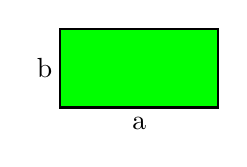
\begin{tikzpicture}[style=thick, fill=green]
        \draw[fill=green] (0,0) rectangle (2,1);
        \draw             (1.0, -0.2) node{a};
        \draw             (-0.2, 0.5) node{b};
      \end{tikzpicture}
    \end{center}
  \end{minipage}%
  \begin{minipage}{0.45\linewidth}
    $A = a \cdot b$
  \end{minipage}
  \pause
  \begin{minipage}{0.45\linewidth}
    \begin{center}
      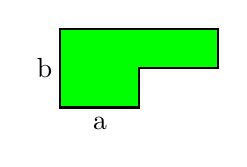
\begin{tikzpicture}[style=thick]
        \path[draw,fill=green] (0,0) -- (1,0) -- (1,0.5) -- (2, 0.5)
           -- (2,1) -- (0,1) -- cycle;
        \draw             (0.5, -0.2) node{a};
        \draw             (-0.2, 0.5) node{b};
      \end{tikzpicture}
    \end{center}
  \end{minipage}%
  \begin{minipage}{0.45\linewidth}
    $A = a \cdot b + \tfrac12 a \cdot b = \tfrac 32 \cdot a \cdot b$
  \end{minipage}

  \begin{minipage}{0.45\linewidth}
    \begin{center}
      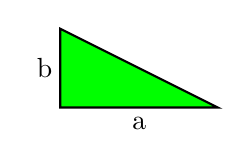
\begin{tikzpicture}[style=thick]
        \path[draw,fill=green] (0,0) -- (2,0) -- (0,1) -- cycle;
        \draw             (1.0, -0.2) node{a};
        \draw             (-0.2, 0.5) node{b};
      \end{tikzpicture}
    \end{center}
  \end{minipage}%
  \begin{minipage}{0.45\linewidth}
    $A = \tfrac12 a \cdot b$
  \end{minipage}



\end{frame}

\begin{frame}{Why Measure Theory?}
  \begin{minipage}{0.45\linewidth}
  \begin{center}
    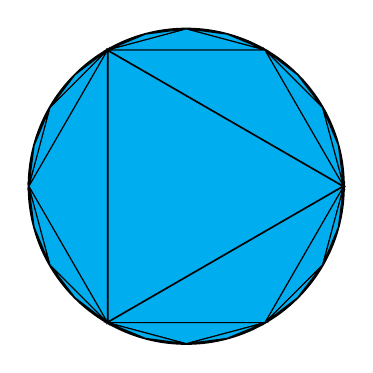
\begin{tikzpicture}[style=thick]
      \draw[fill=green] (0,0) circle (2);
      \pause
     % \draw             (1.0, -0.2) node{a};
      \path[draw,fill=cyan] (0:2)
      \foreach \x in {120,240}
        { -- (\x:2) } -- cycle;
      
      %\foreach \y in {0, 120, 240}
      %{
      %  \path[draw,fill=cyan] (\y:2)
      %  \foreach \x in {0,60,120}
      %   { -- (\x+\y:2) } -- cycle;
      %}
      \foreach \k in {3,6,12}
      { 
        \pause
        \foreach \x [evaluate=\x as \xx using (\x-1)*360/\k] in {1, ..., \k}
        { \path[draw,fill=cyan,style=thin] (\xx:2) 
          %\node{\x} at (\xx:2);
          \foreach \y [evaluate=\y as \yy using \xx+\y*360/\k/2] in {0,1,2}
          { -- (\yy:2) }
          -- cycle;
        }
      }
     \end{tikzpicture}
  \end{center}
  \end{minipage}%
  \begin{minipage}{0.45\linewidth}
    $\only<2-5>{A \leq A_1}
       \only<3-5>{+ 3A_2}
       \only<4-5>{+ 6 A_3}
       \only<5-5>{+ 12 A_4}$
    $\only<6>{A = A_1 + 3\sum_{n=0}^\infty 2^n A_{n+2}}$
  \end{minipage}
\end{frame}


\begin{frame}{Why Measure Theory?}

  \begin{itemize}
  \item Ca. 1900: What is a volume?
    \begin{definition}
      A volume is a function $\mathcal{P}(\RR^n) \to [0, \infty]$ such that
      \begin{enumerate}
      \item Positivity: $\mu_n(A) \geq 0$ for all $A \subset \RR^n$.
      \item Kongruence: $\mu_n(A) = \mu_n(B)$ for all kongruent $A$ and $B$.
      \item Norm: $\mu_n([0,1]^n) = 1$.
      \item $\sigma$-Additivity: $\mu_n(\bigcup_{i=1}^{\infty} A_i) =
        \sum_{i=1}^\infty \mu_n(A_i)$ for disjoint $A_i$.
      \end{enumerate}
    \end{definition}
    \begin{lemma}
      \begin{enumerate}
      \item $\mu_n(\{x\}) = 0$
      \item $\mu_n(A) \leq \mu_n(B)$ for $A \subseteq B$.
      \end{enumerate}
    \end{lemma}

  \end{itemize}



\end{frame}

\begin{frame}{The vitali set}
  Let $V$ be a set of representatives for the quotient group $\RR/\QQ$
  from $[0,1]$, that is: For every $z \in \RR$, there is exactly one
  element of $z+\QQ$ in $V$ and this element lies in $[0,1]$.

  \begin{lemma}
    \begin{enumerate}
    \item For $p\neq q$, $p,q\in\QQ$ and for a enumeration of the we
      have $p+V \cap q+V = \emptyset$.
    \item Let $(p_n)_{n\in\NN}$ an enumeration of the rational numbers
      in $[-1,1]$ and $V_n=p_n + V$, then we have $[0,1] \subset
      \bigcup_{n=1}^{\infty} V_n \subset [-1, 2]$.
    \end{enumerate}
  \end{lemma}
\end{frame}

\begin{frame}{The Vitali set}

  We have by monotony
  
  \[1 \leq \sum_{n=1}^\infty \mu_1(V_n) \leq 3\]

  but by congruence we have $\mu_1(V_n) = \mu_1(V)$ for all $n$, therefore

  \[1 \leq \sum_{n=1}^\infty \mu_1(V) \leq 3\]

  But if $\mu_1(V)=0$ then $\sum_{n=1}^\infty \mu_1(V)=0$ and if
  $\mu_1(V)>0$ then $\sum_{n=1}^\infty \mu_1(V) = \infty$. Therefore
  such a $\mu_1$ cannot exist.

\end{frame}


\section{Measure Theory}

\section{Probability Theory}


\end{document}
